%======================================================================
\chapter{Introduction}
%======================================================================
Nuclear fusion, the process by which two light atomic nuclei combine to form a heavier nucleus, holds the promise of revolutionizing the world's energy landscape. With the ever-increasing demand for sustainable, clean, and virtually limitless energy sources, nuclear fusion has emerged as a leading candidate. Nuclear fusion, in contrast to the fission processes used in current nuclear power plants, presents a fundamentally safer and more sustainable option. The primary fuel for fusion, isotopes of hydrogen, is abundant and can be extracted from water sources. Fusion reactions produce no long-lived, highly radioactive waste, minimizing environmental hazards and long-term disposal issues. Recent advancements have reignited interest in the field, with notable breakthroughs such as the development of high-temperature superconducting magnets, which enable the efficient confinement of high-energy plasma. An excellent example is the rare earth barium copper oxide high-temperature superconducting magnets that are being deployed in the SPARC experimental reactor \cite{SPARCoverview}. In February 2022, the UK-based JET laboratory reported that it had smashed its own world record for the amount of energy it could extract by squeezing together two forms of hydrogen, deuterium and tritium. The experiments produced 59 megajoules of energy over five seconds (11 megawatts of power), which was more than double what was achieved in similar tests back in 1997. Another breakthrough was announced in December 2022 by US scientists at the National Ignition Facility in California. They confirmed that they had achieved ignition for the first time, by firing up to 192 giant lasers into a peppercorn-sized fuel pellet and triggering a fusion reaction that released more energy than was put in by the lasers \cite{nationalignitionfacilitycali}.

\begin{figure}[H]
    \centering
    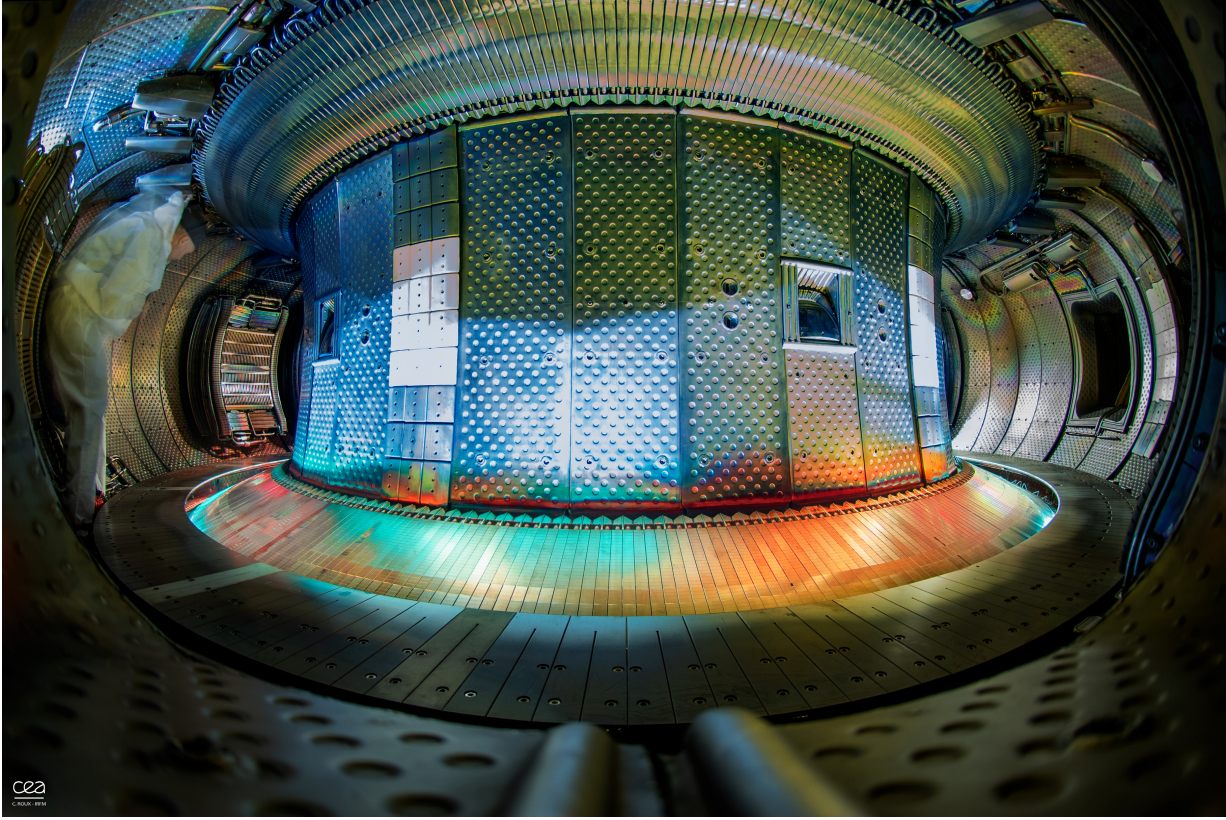
\includegraphics[width=\textwidth]{images/Final/vaccumeVessel.jpg}
    \caption{The vacuum vessel that holds magnetically confined plasma within the WEST tokamak \cite{vacves}.}
    \label{fig:vacves}
  \end{figure}

Tokamaks are a class of fusion devices with great potential to achieve commercial fusion energy production. Tokamaks use magnetic fields to confine and heat plasma, a state of matter where atoms are split into electrons and nuclei. The immense pressures and temperatures created induce fusion reactions between light nuclei, such as hydrogen, to produce energy. Tokamaks currently demonstrate long plasma confinement times, which measure how well the plasma is isolated from the surrounding environment and affect the efficiency of energy production and heat loss. Tokamaks have the most extensive scientific and technological knowledge base, which has been accumulated over decades of research and development. This leads to reliable and robust designs, advanced diagnostics and control systems, and proven solutions for engineering challenges. These advantages make tokamaks the most promising candidates for achieving commercial fusion energy in the near future. Tokamaks have already shown impressive results in terms of fusion power output and energy gain. They are expected to reach even higher levels of performance with the next generation of devices. Tokamaks are also supported by a strong international collaboration and a clear roadmap for development. Therefore, tokamaks have a huge potential to commercialise fusion before other methods: especially with ITER just around the corner and plans for DEMO already underway. ITER and DEMO are complementary projects that will advance fusion energy from the experimental stage to the commercial stage. ITER will provide the scientific and technological basis for DEMO, which will be the first fusion power plant to produce electricity and operate with a closed fuel cycle. The construction of ITER is expected to be completed by 2025, and the first plasma operation is planned for 2026. The full deuterium-tritium operation of ITER is scheduled for 2035, which will coincide with the start of the construction of DEMO. The operation of DEMO is foreseen to begin in the 2040s, and to demonstrate the viability of fusion energy for commercial use.

The electron density profile is a key parameter that affects the performance and stability of tokamak plasmas. It affects the plasma current, the confinement time, the energy transport, the magnetohydrodynamic (MHD) modes, and the coupling of external heating and current drive sources. There are physical limits that constrain the maximum achievable density in tokamak plasmas. One of the most well-known density limits is the Greenwald limit, which states that the line-averaged density cannot exceed a value proportional to the plasma current divided by the plasma cross-sectional area. This limit is empirically observed in many tokamaks, and attempts to exceed it result in disruptions or edge localized modes (ELMs). The physical mechanism behind the Greenwald limit is not fully understood, but it may be related to the stability of the edge pedestal, the bootstrap current, or the core particle transport. A lower electron density leads to runaway electrons. The magnetic fields accelerate the electrons continuously and only collisions prevent them from gaining enough energy to escape the magnetic confinement. A low density can mean that collisions are not frequent enough to prevent escape and the electrons can cause serious damage to the plasma facing wall. Thus it is not beneficial for the plasmas electron density profile to be such as to have many electrons with a low density near the edge. 

One of the main challenges in measuring the electron density profile is to obtain high spatial and temporal resolution over a wide radial range. Several diagnostic techniques have been developed and applied to tokamaks, such as interferometry, reflectometry, Thomson scattering, and spectroscopy. Each technique has its own advantages and limitations in terms of accuracy, reliability, coverage, and invasiveness. A combination of different techniques is often used to obtain a comprehensive picture of the electron density profile evolution.

Another worthy challenge is to maintain the electron density profile in a desired shape. The electron density profile is influenced by various factors, such as plasma geometry/magnetic configuration, plasma current and pressure, impurity content, fueling and pumping methods, and external heating and current drive sources. Some of these factors can be manipulated by the operators, others can be controlled in real time with sophisticated algorithms and feedback loops; achieving a favourable electron density profile that enhances the plasma performance and stability.

The electron density profile is an important parameter that determines many aspects of tokamak plasmas. Measuring and controlling the electron density profile is a crucial task for optimizing the tokamak operation and achieving fusion energy goals.

This thesis focuses on performing a Bayesian inference of the electron density profile using the interferometry diagnostic and a Gaussian process prior. Bayesian inference with a Gaussian process prior is a powerful technique for the nonparametric modelling of complex phenomena. A Gaussian process is a collection of random variables, which have a joint Gaussian distribution. A Gaussian process can be specified by a mean vector and a covariance matrix. By applying Bayes’ rule, one can obtain the posterior distribution for an unknown profile, given some observed data. The posterior can be used for prediction and uncertainty quantification. Interferometry is a technique that uses the interference of electromagnetic waves to measure the properties of a medium. The interferometer within a tokamak consists of many laser beams penetrating the plasma at various angles. This thesis uses the \gls{west} tokamak's laser geometry which covers a span of the poloidal cross section. Although there is not enough information to completely and accurately reconstruct the electron density profile a best guess given the data can be inferred. For real data, it is difficult or impossible to know how close any inferred profile is to the true profile.

Bayesian integrated analysis is often used to combine multiple diagnostics which measure the same or related physical parameters. This involves combining multiple diagnostics with the Bayesian framework which provides a universal way to treat uncertainties of any probability density function. R Fischera from the Max-Planck-Institut für Plasmaphysik published a paper on using Bayesian integrated analysis with Thomson scattering, interferometry and lithium beam diagnostics to combine their information on the electron density profile \cite{IDAmaxPlanck}. They focused on obtaining a systematic and formalized error analysis of all uncertainties involved in each diagnostic. These are then quantified within the likelihood. Jiahong Chen published a paper on the development of a Bayesian integrated analysis program developed for the HL-2A tokamak \cite{IDAgeert2023}. For the electron density profile, it combines interferometry and reflectometry. It aims to infer a 2D profile whilst this thesis focuses on a 1D profile. The program is a full Bayesian analysis from the raw data to the results. This thesis also aims to go from raw interferometry data to results in a fully Bayesian way. GT von Nessi and MJ Hole also published a paper on the combination of interferometry and Thompson scattering to infer the electron density and temperature profile with Bayesian inference and Gaussian Processes \cite{nessiIBAmega-ampere-spherical}. Their work mainly focuses on the Thompson scattering diagnostic. Interferometry is not used to determine the shape of the profile but to contain the magnitude of the electron density given a profile shape. This avoids the difficult calibration of the integrated Thompson beam energy.  

There is a common rhythm to these papers that is also echoed in my thesis. The problem is broken down with Bayes' theorem and the form of the various distributions are identified or defined. A forward model is defined that allows one to obtain an error free version of the data given a defined ground truth of the physical quantity of interest. The forward model is essential to computing the likelihood. The hyperparameters and their priors are identified and optimised using the hyperparameter \gls{map} method or marginalisation. The posterior is computed with analytical expressions where possible or \gls{mcmc} techniques are used to sample from the posterior. The posterior is presented as a probability distribution showing the most likely values of the physical quantity of interest and its uncertainty. There are many caveats and details that are specific to each implementation yet the overarching story remains intact. This thesis does not aim to combine multiple diagnostics but focuses on interferometry. The goal is to use raw interferometry data to infer the electron density profile with Bayesian techniques. 

The background theory chapter introduces the tokamak and some necessary physics required to understand the assumptions made. The \gls{west} tokamak has implemented \gls{nice} code to reconstruct the magnetic equilibrium and it also outputs the electron density profile as a byproduct. A brief description of \gls{nice}'s method is provided for comparison to the techniques in this thesis. Bayesian inference with Gaussian processes is introduced for a simple regression problem. It is introduced in such a way that the step to inferring the electron density profile from interferometry can be done simply by changing the forward model used. Some more advanced alterations to the process are explained to include further assumptions of the problem. Interferometry is explained in enough detail to understand how the density profile information is present within the data. The procedures explained in the background theory are then applied to synthetic interferometry data that was created with a ground truth profile assumption. This allows for a precise quantification of the performance through the mean square error. All of H mode, L mode and peaking are explored through synthetic data. Real interferometry data is taken from the \gls{west} tokamak and the resulting inferred profiles can be compared to \gls{nice}. 

% write about whats included in each chapter, 

% then summarise the introduction

% maybe reword somethings to sound like yourself a bit more. Tone down some of the scientific claims/ add refferences.

% Add some images to make it more lively. Possibly a nice fuision of whatever fuses in west. 




% Introduce the main concepts, ideas and motivation. Include a small literature review on related works, including \gls{nice} and \gls{west}. Introduce the outline of the thesis.

% % \begin{itemize}
% %     \item introduce magnetic confinement fusion, the tokamak and the electron density profile
% %     \item Justify topic, why the electron density profile is important, why interferometry is a good diagnostic, why Bayesian inference is good in particular \gls{gpr}. How this can be expanded to combine other diagnostics in an bayesian integrated analysis. 
% %         \subitem{Quality of confinement ie distinguishes between H and L mode}
% %         \subitem{Key role in ignition criteria, explain section from Wesson Tokamaks}
% %         \subitem{Operation limits, Low density electrons can run away, high density over greenwald limit leads to instabilities. I imagine H-mode reduces runaway electrons}
% %     \item give the details of the WEST tokamak and the IMAS database system. 
% %     \item explain that NICE exists and that it will be the main source of comparison
% %     \item Summarise all work in a few paragraphs
% %     \item Give a literature review on what is the current status of the research in this topic.
% %         \subitem{Cholinskey Thompson Scattering implementation of \gls{gpr}.}
% %         \subitem{Show rough number on papers using GPR in fusion, perhaps a history of it.}
% %         \subitem{What other diagnostics can be used, how many have papers that use a \Gls{gpr} analysis?}
% %         \subitem{What are the other inference algorithms for accomplishing the same goal. I imagine for each diagnostic the algorithm is very different whilst bayesian methods are more widly applicable, GPR can be used for every diagnostic with a linear forward model and monte carlo sampling techniques can be used for all of them, thus simplifying the field.}
% %     \item Describe what is in the other sections of the thesis
% % \end{itemize}



